\documentclass{beamer}
\usetheme{Madrid}
\usecolortheme{default}
\usepackage[T1]{fontenc}
\usepackage[french]{babel}
\usepackage{graphicx}
\usepackage{amsmath}
\usepackage{amssymb}
\usepackage{mathrsfs}

% Ajouter le plan en haut
\useoutertheme{infolines}
\setbeamertemplate{headline}{
	\begin{beamercolorbox}[ht=2.25ex,dp=3.75ex]{section in head/foot}
		\insertnavigation{\paperwidth}
\end{beamercolorbox}}

\title[]
{Atténuation des vibrations grâce à
	un amortisseur harmonique passif}

\subtitle{}

\author{Noé Bocquillon} % (optional, for multiple authors)




\date[n°20041] % (optional)
{Numéro de candidat:\\ 20041}

%\logo{\includegraphics[height=0.8cm]{logo_uoft}}

\definecolor{uoftblue}{RGB}{6,41,88}
\setbeamercolor{titlelike}{bg=uoftblue}
\setbeamerfont{title}{series=\bfseries}
\setbeamertemplate{caption}[numbered]
\begin{document}
	
	\frame{\titlepage}
	\section{Préambule}
	\begin{frame}{Préambule}
		\frametitle{Introduction}
		
		
		\begin{columns}[T]
			\begin{column}{0.45\textwidth}
				\begin{figure}
					\centering
					\includegraphics[width=\textwidth]{C:/Users/noebo/OneDrive/Documents/Prépa/TIPE TMD/Présentation/Photos/image tmd pont}
					\caption{Tuned mass damper sur un pont}
				\end{figure}
				
			\end{column}
			\begin{column}{0.45\textwidth}
				\begin{figure}
					\centering
					\caption{ Pendule de la tour Tapei 101 à Taiwan}
					\includegraphics[width=\textwidth]{C:/Users/noebo/OneDrive/Documents/Prépa/TIPE TMD/Présentation/Photos/image tour tawai pendule}
				\end{figure}
			\end{column}
		\end{columns}
		\bigskip\small TMD = Tuned mass damper
	\end{frame}
	
	%\section{First section}
	\begin{frame}{Préambule}
		\frametitle{Objectifs}
		\underline{Problématique:} Quelle est l'influence du Tuned Mass Damper lors d'une excitation extérieure ? 
		\vspace{12pt}
		\linebreak[3]Objectifs du TIPE:
		\begin{itemize}
			\item\ Modéliser un immeuble subissant une contrainte extérieure
			\item Étudier l'influence du TMD et de ses paramètres sur l'atténuation des vibrations de la maquette
			
		\end{itemize}
		
	\end{frame}
	
	\begin{frame}{Plan}
		\begin{enumerate}
			\item\huge{Construction de la maquette et développement de l'outil de vibration} \linebreak
			\item Mise en vibration de la maquette\linebreak
			\item Élaboration d'un modèle théorique et conclusion 
		\end{enumerate}
	\end{frame}
	
	\section{Construction de la maquette}
	\begin{frame}{Construction de la maquette}
		Schéma global du système
		\begin{columns}
			\begin{column}{0.3\textwidth}
				\begin{figure}
					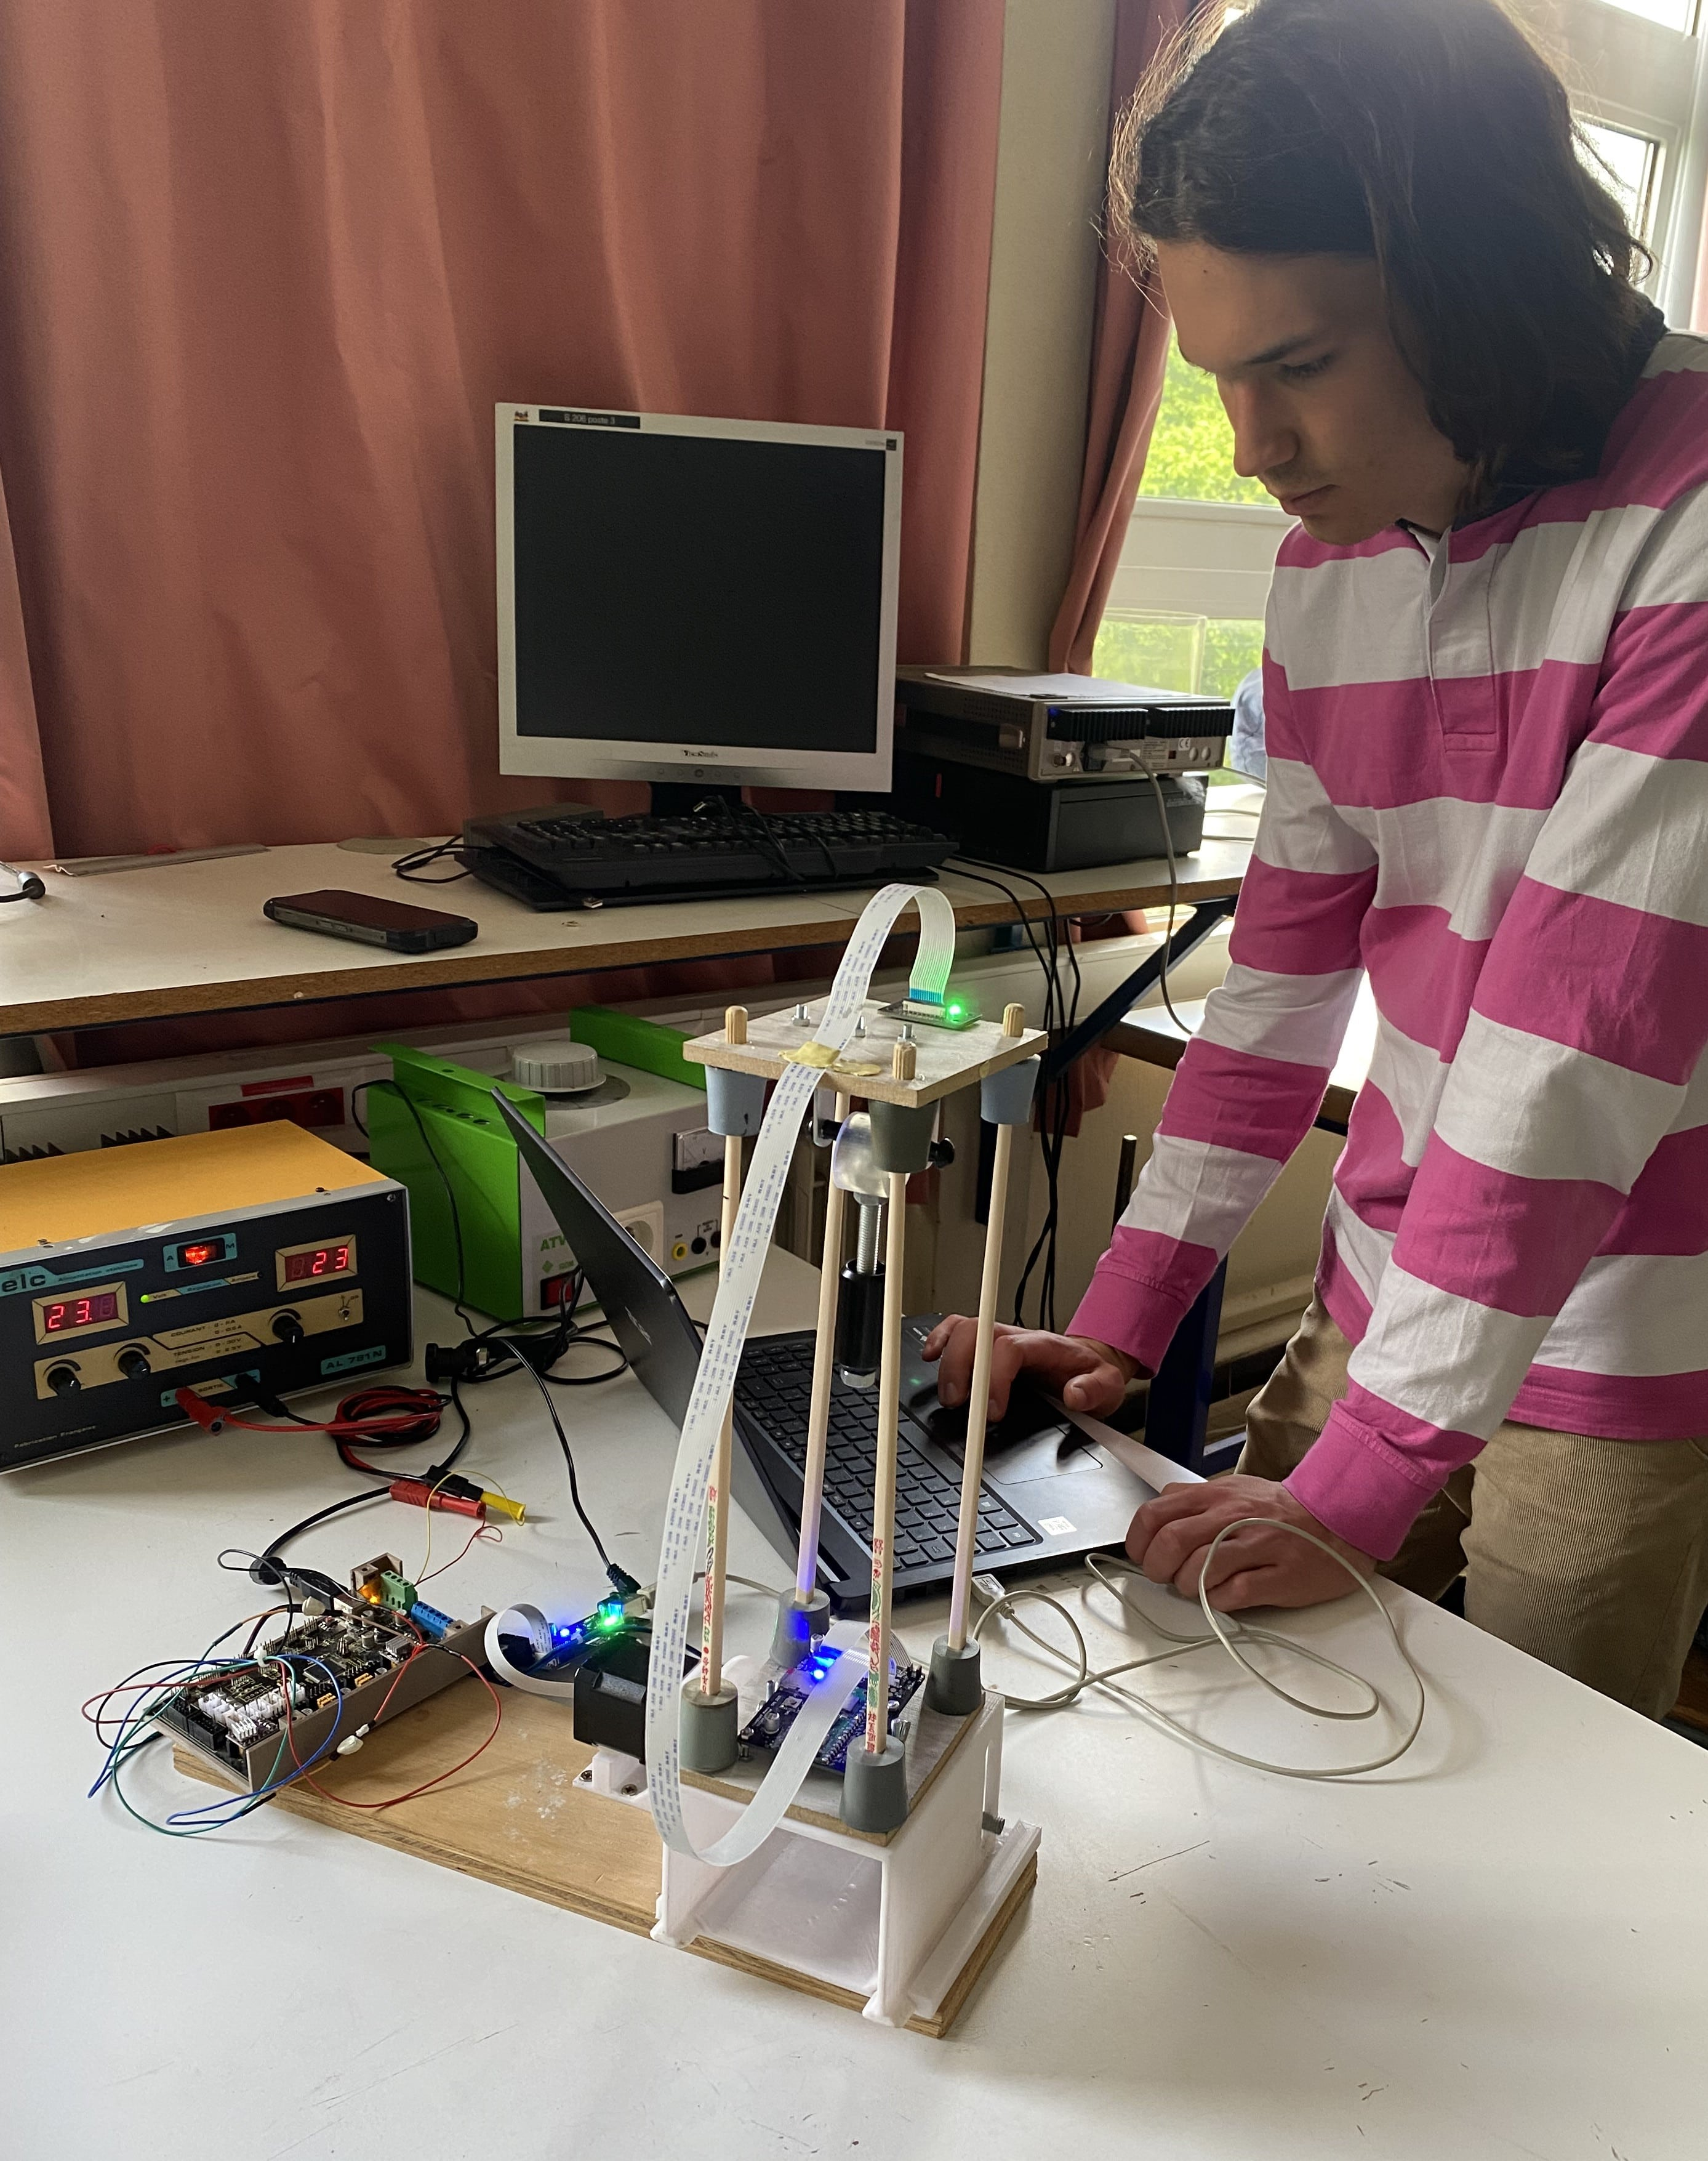
\includegraphics[width=\textwidth]{C:/Users/noebo/OneDrive/Documents/Prépa/TIPE TMD/Présentation/Photos comp/IMG_3412-min.JPG}
					\caption{Montage global}
				\end{figure}
				%Changer photo , plus global plus zoom
			\end{column}
			\begin{column}{0.3\textwidth}
			
			\begin{figure}
				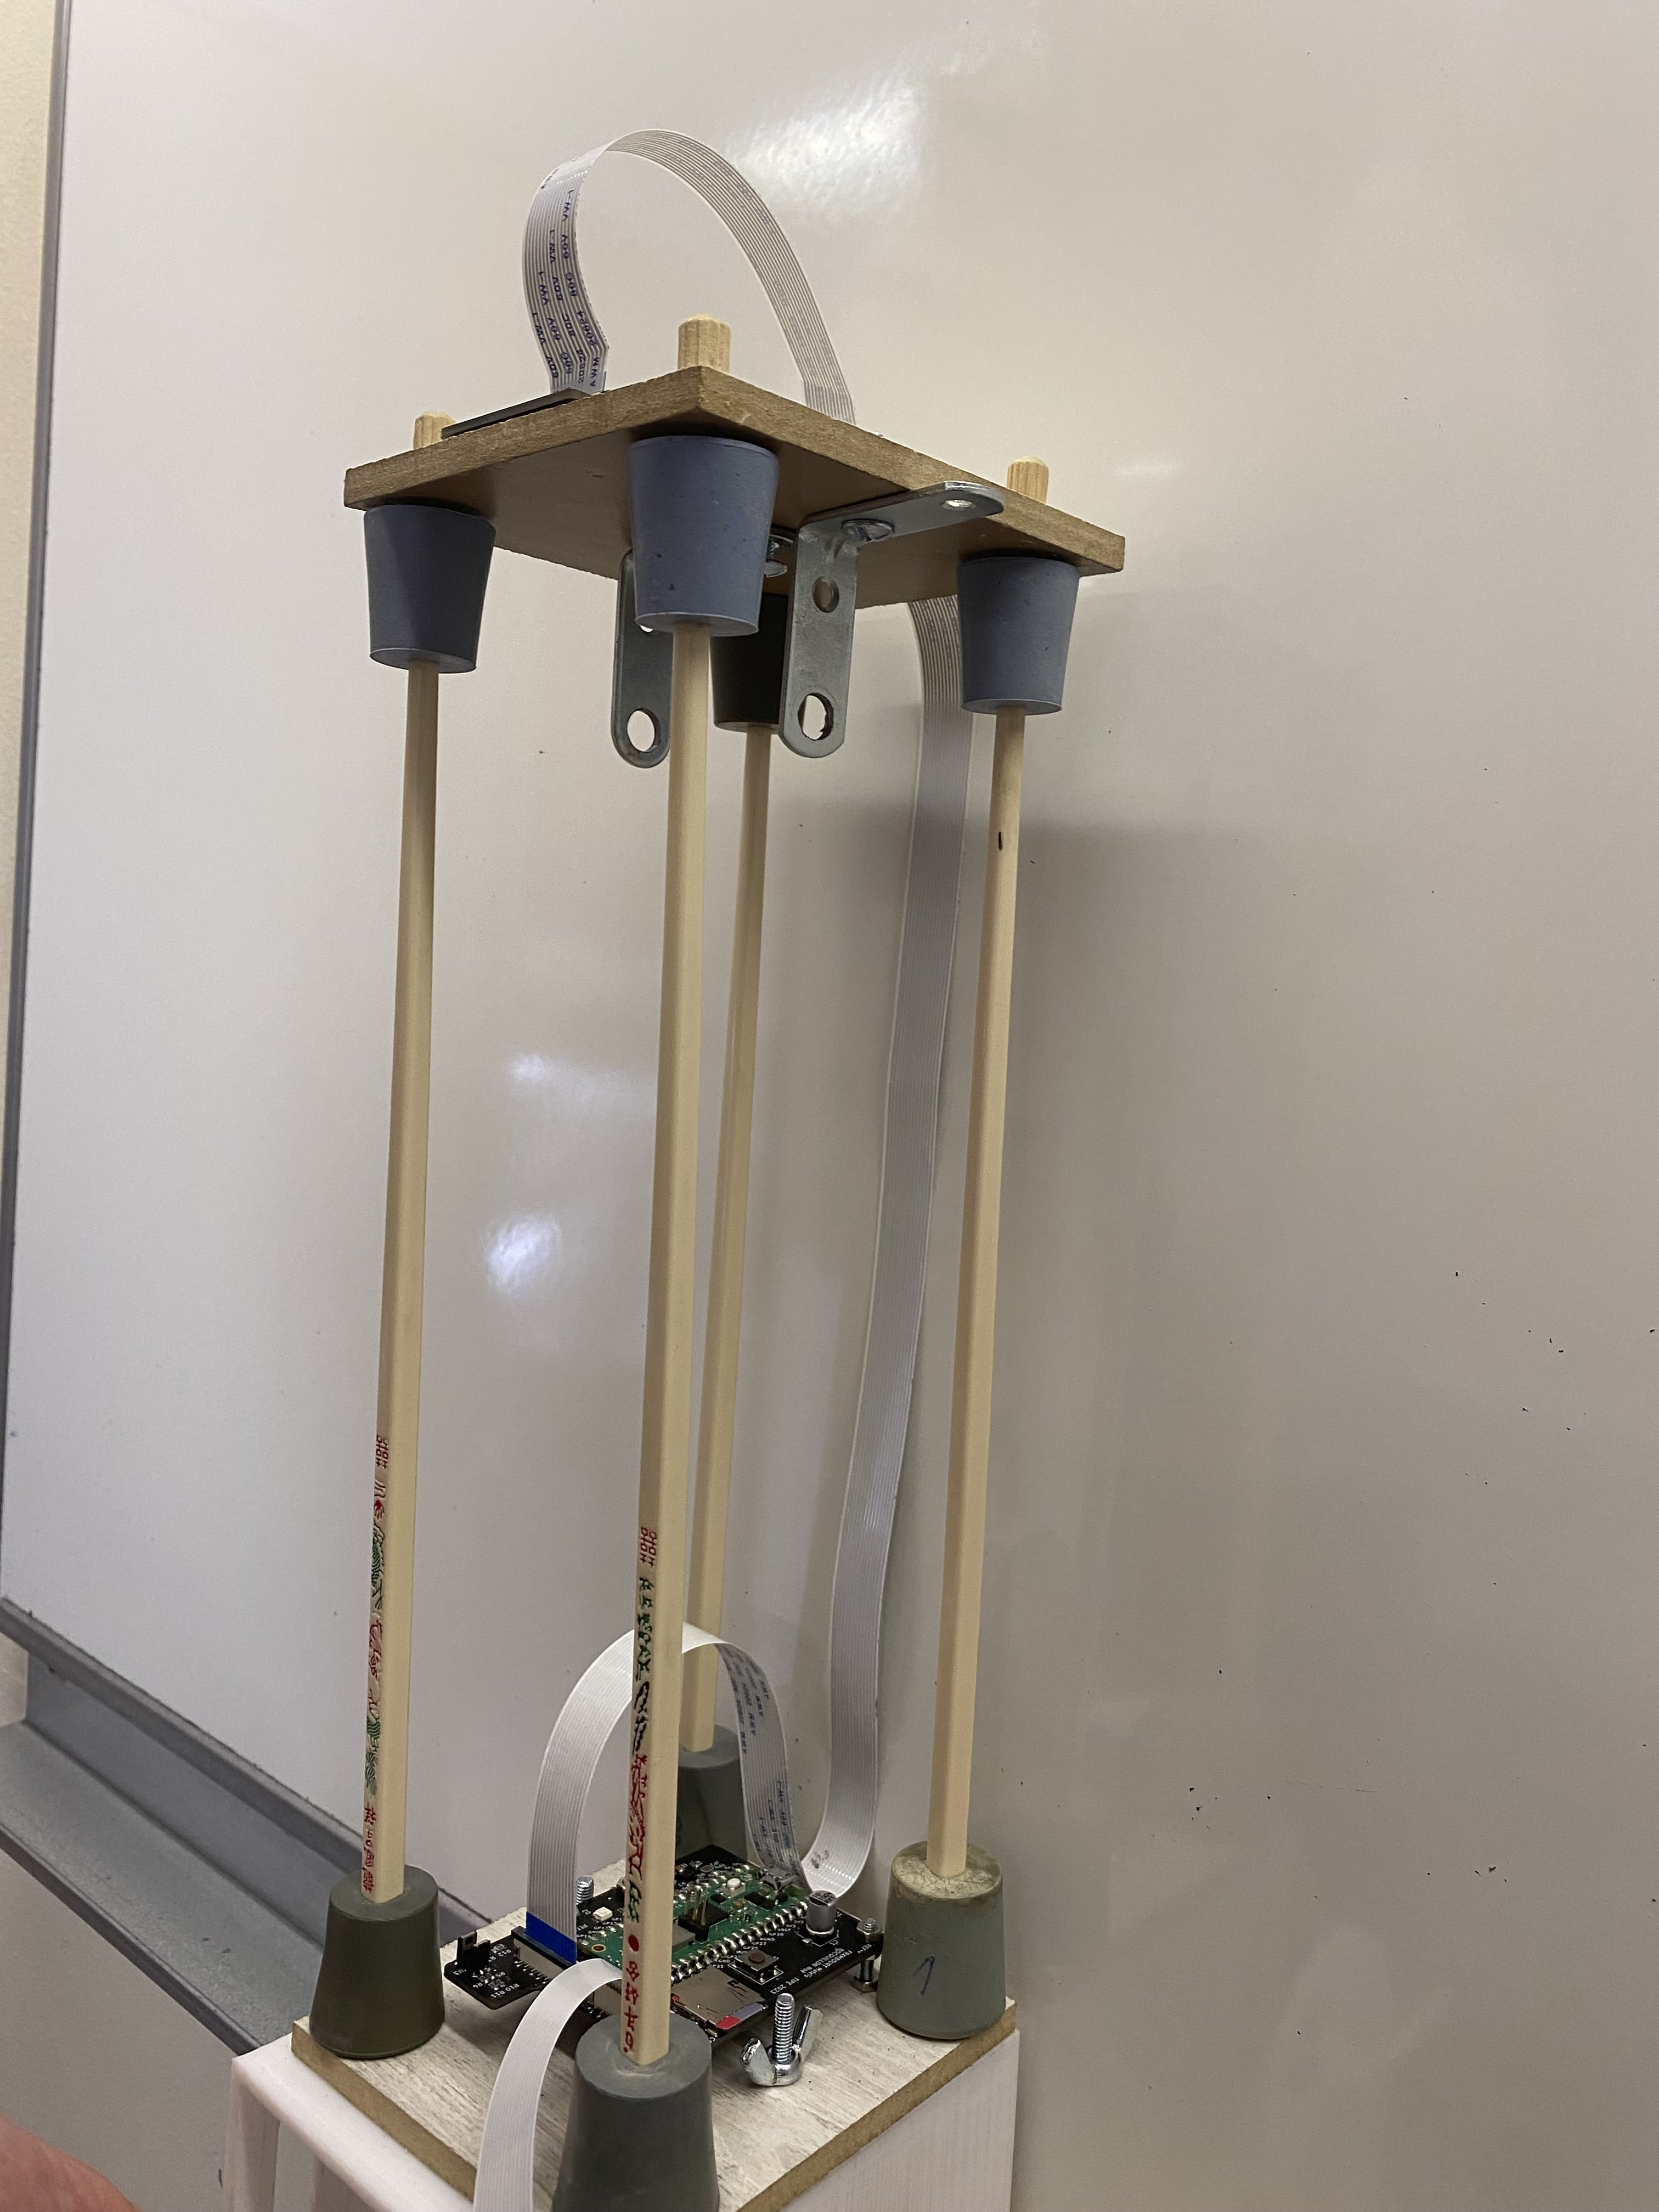
\includegraphics[width=\textwidth]{C:/Users/noebo/OneDrive/Documents/Prépa/TIPE TMD/Présentation/Photos comp/IMG_3380-min.JPG}
				\caption{Maquette de l'immeuble}
			\end{figure}
			\end{column}
	
		\begin{column}{0.2\textwidth}
				Contraintes:
		\begin{itemize}
			\item Taille
			\item Flexibilité \\
		\end{itemize}
		\end{column}
	\end{columns}
	\end{frame}

	
	\begin{frame}{Construction de la maquette}
		\frametitle{Pendule}
		\begin{columns}
			\begin{column}{0,45\textwidth}
				\begin{figure}
					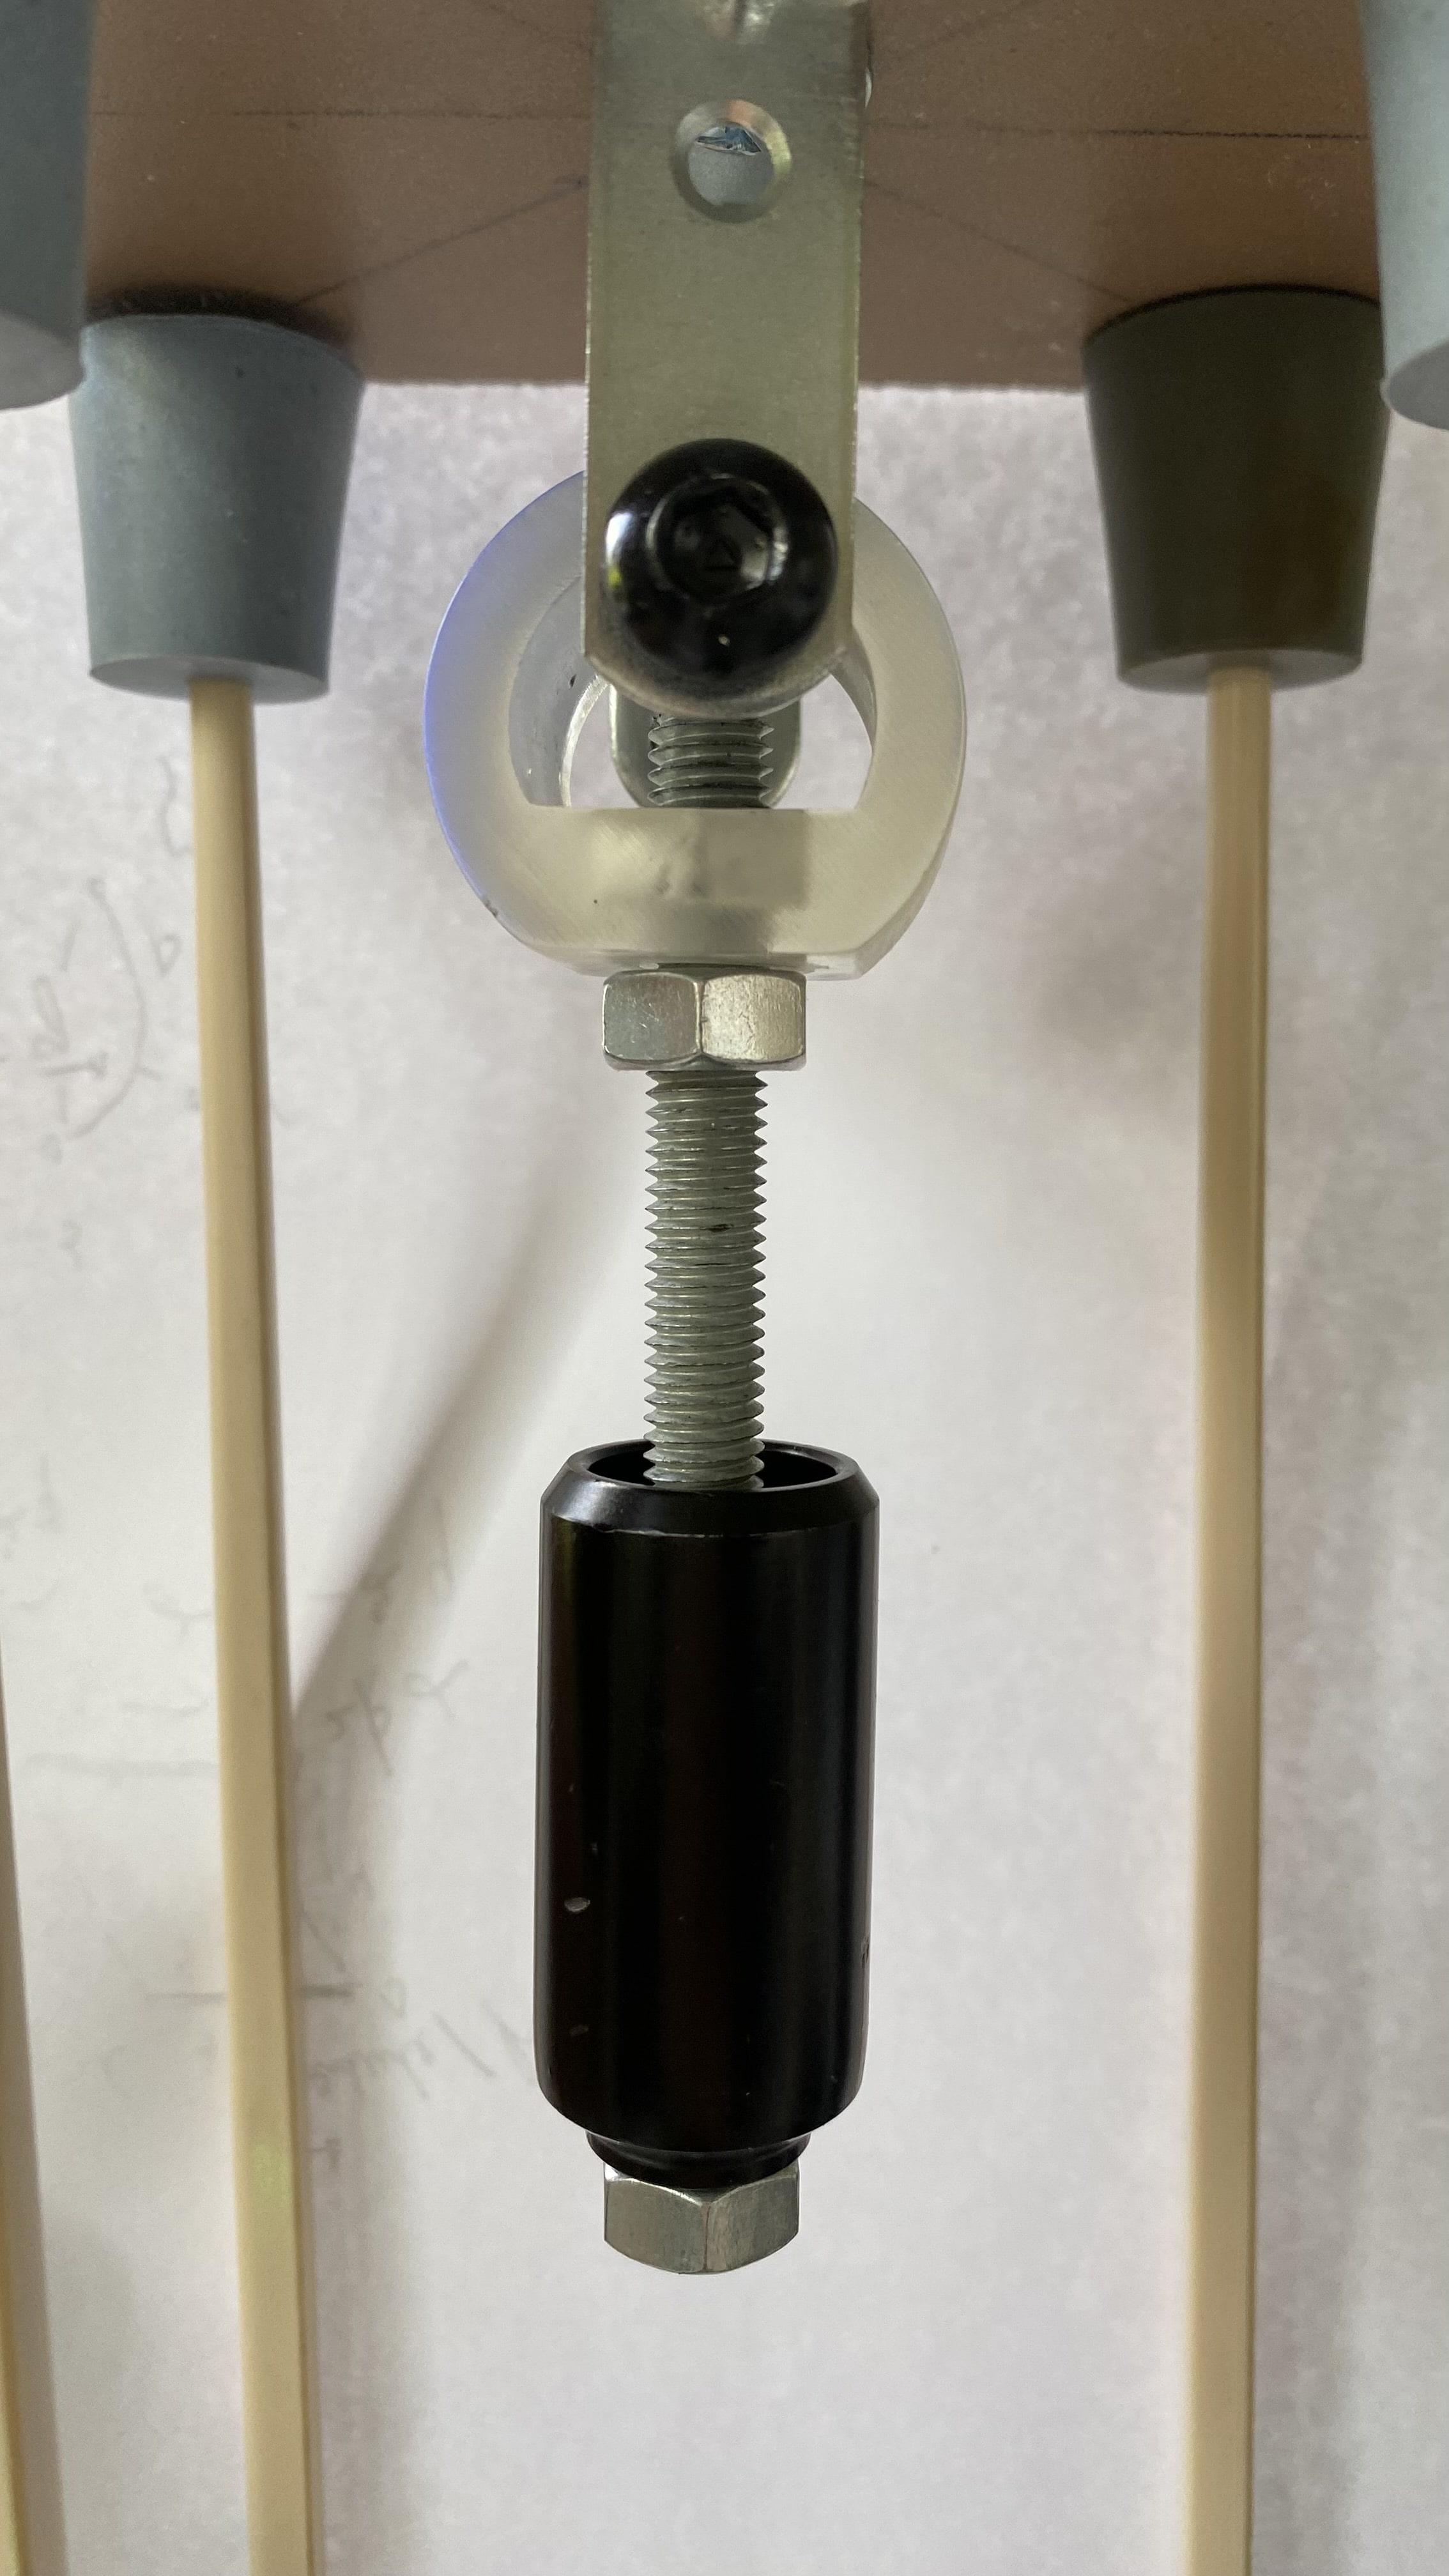
\includegraphics[width=0.6\textwidth]{C:/Users/noebo/OneDrive/Documents/Prépa/TIPE TMD/Présentation/Photos comp/IMG_E3392-min.JPG}
					\caption{Pendule}
				\end{figure}
			\end{column}
		\end{columns}

	\end{frame}

\begin{frame}{Construction de la maquette}
		\frametitle{Outil de mise en vibration}
Un premier échec:
		\begin{columns}
			\begin{column}{0.5\textwidth}
				\begin{figure}
					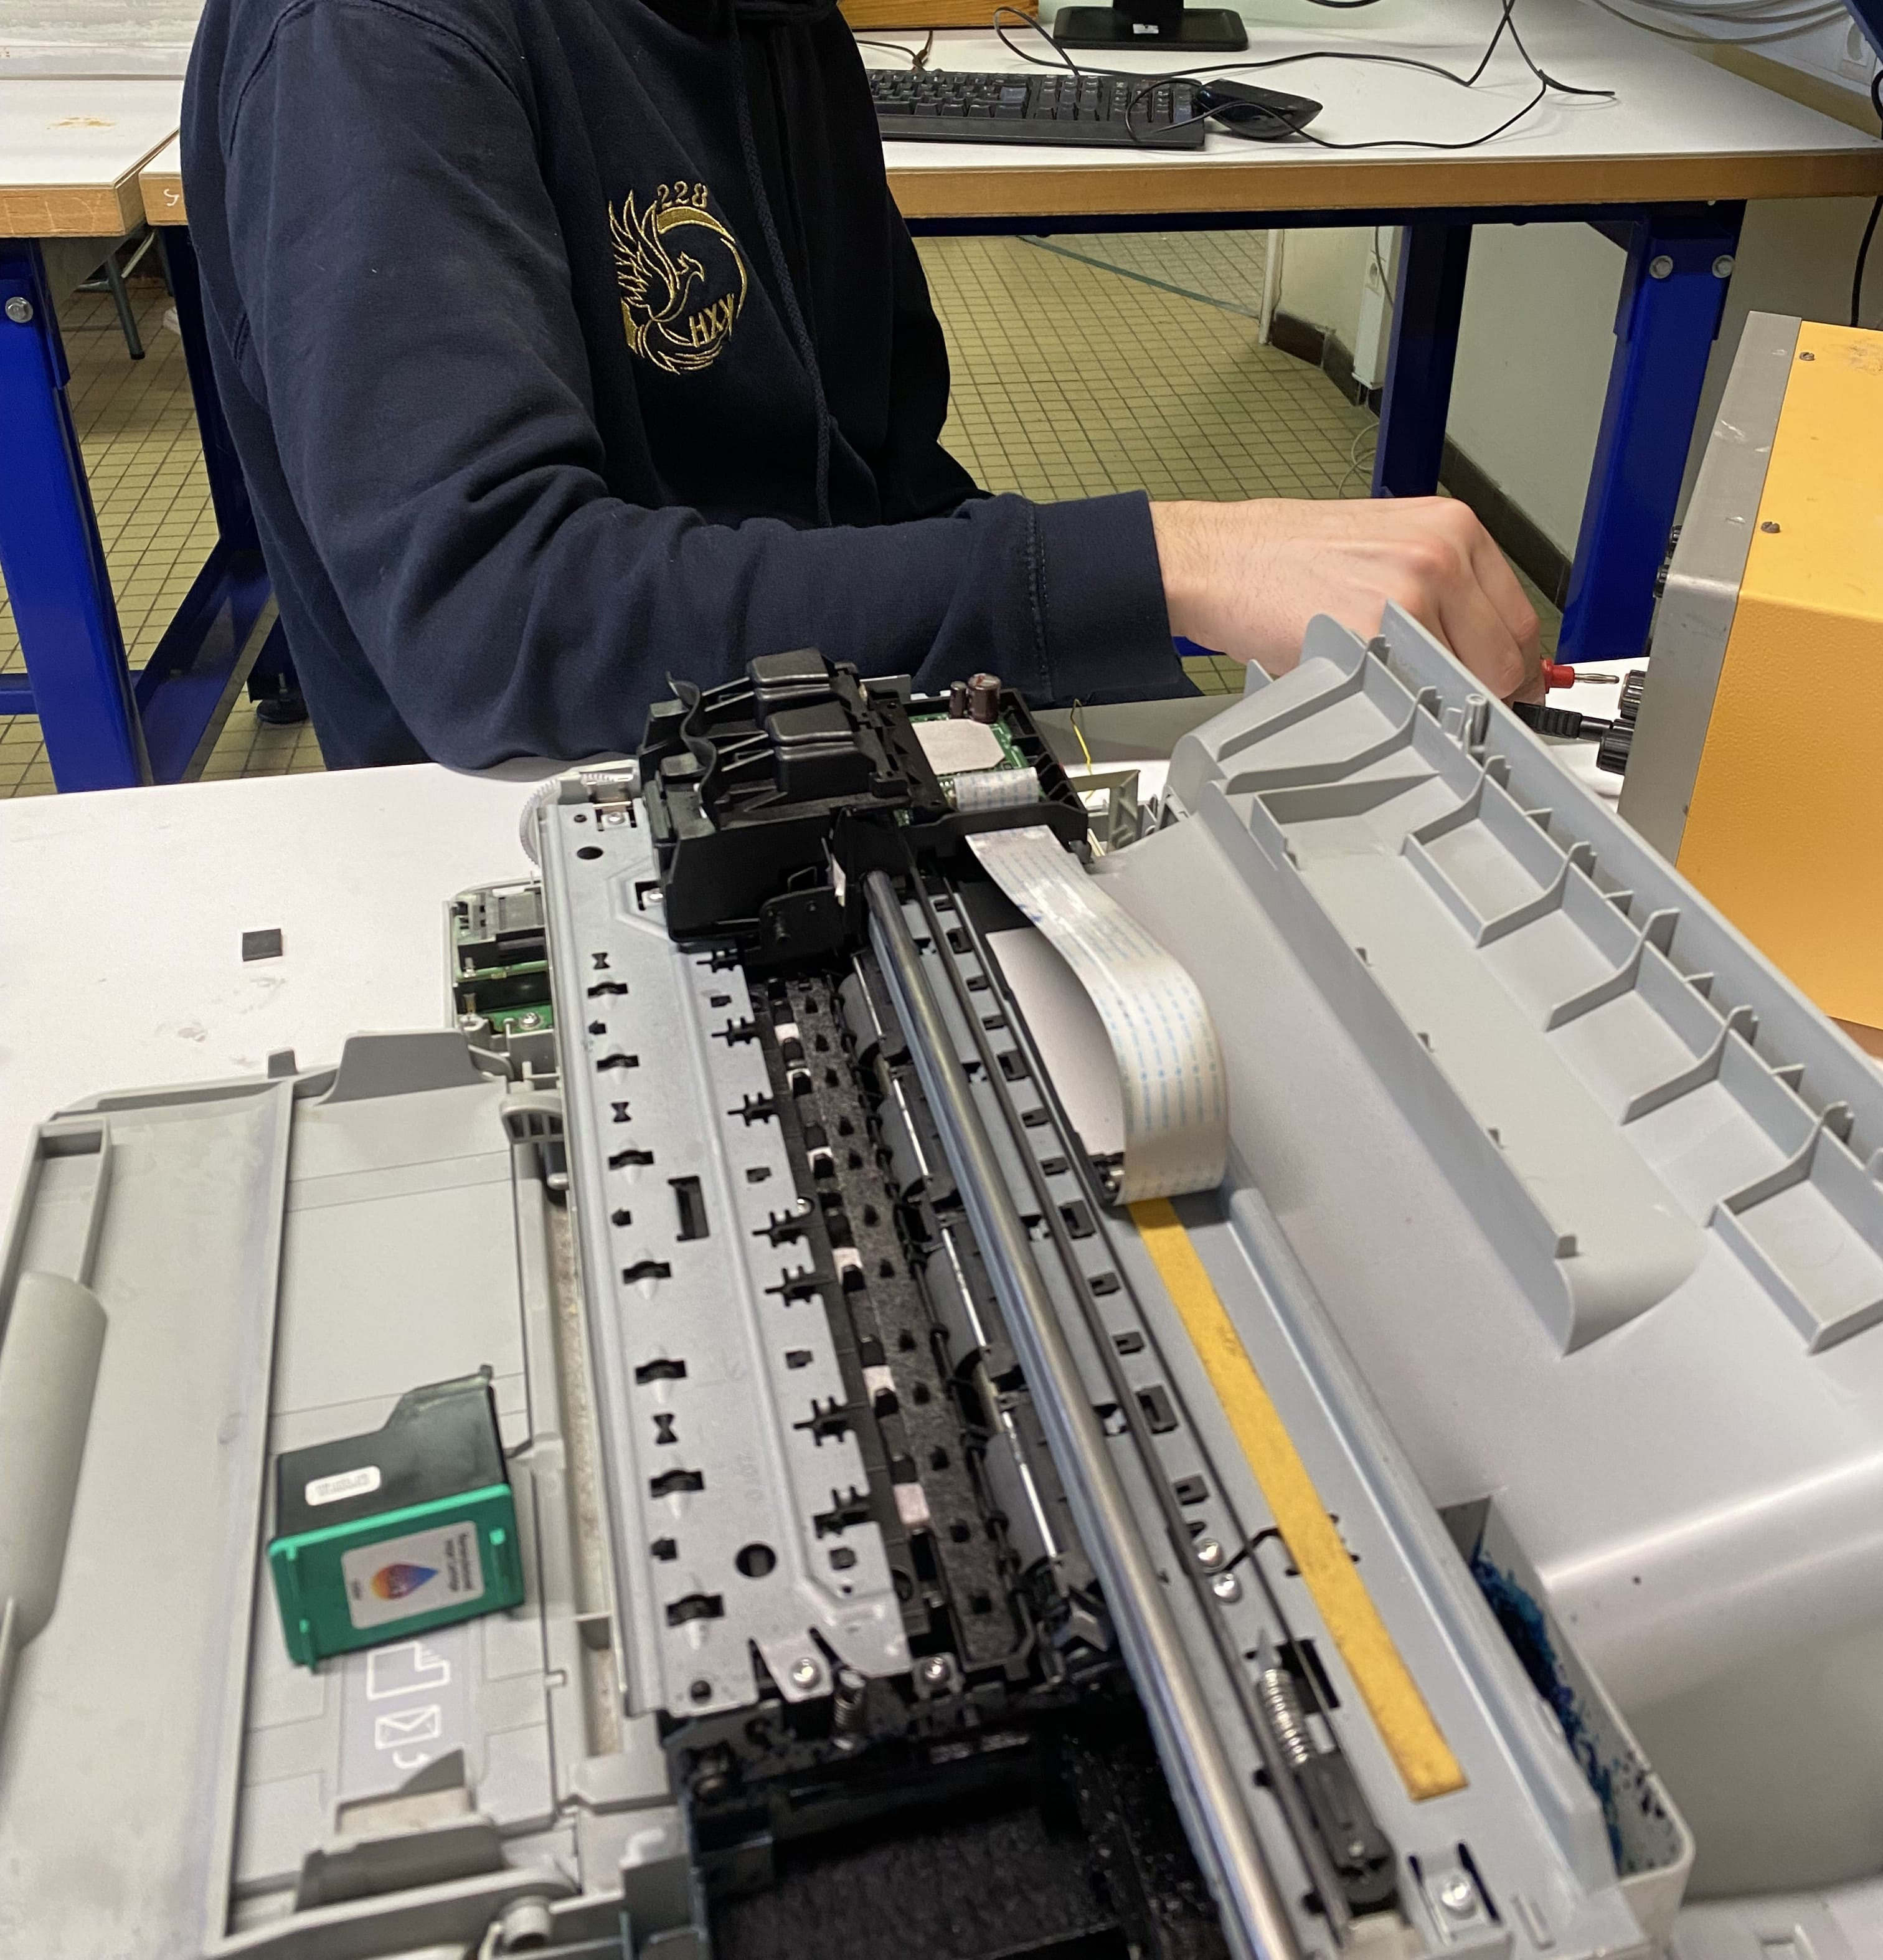
\includegraphics[width=0.8\textwidth]{C:/Users/noebo/OneDrive/Documents/Prépa/TIPE TMD/Présentation/Photos comp/IMG_2609-min.JPG}
					\caption{Guidage en translation d'une imprimante}
				\end{figure}
			\end{column}
			\begin{column}{0.5\textwidth}
				Inconvénients:
				\begin{itemize}
					\item\ difficultés pour fixer la structure
					\item Fréquence non réglable \\
					\item Masse de la structure qui influe sur la vitesse
				\end{itemize}

			\end{column}
		\end{columns}
	\end{frame}
	
	\begin{frame}{Construction de la maquette}
		\frametitle{Outil de mise en vibration}
 
		\begin{columns}
			\begin{column}{0.5\textwidth}
				\begin{figure}
					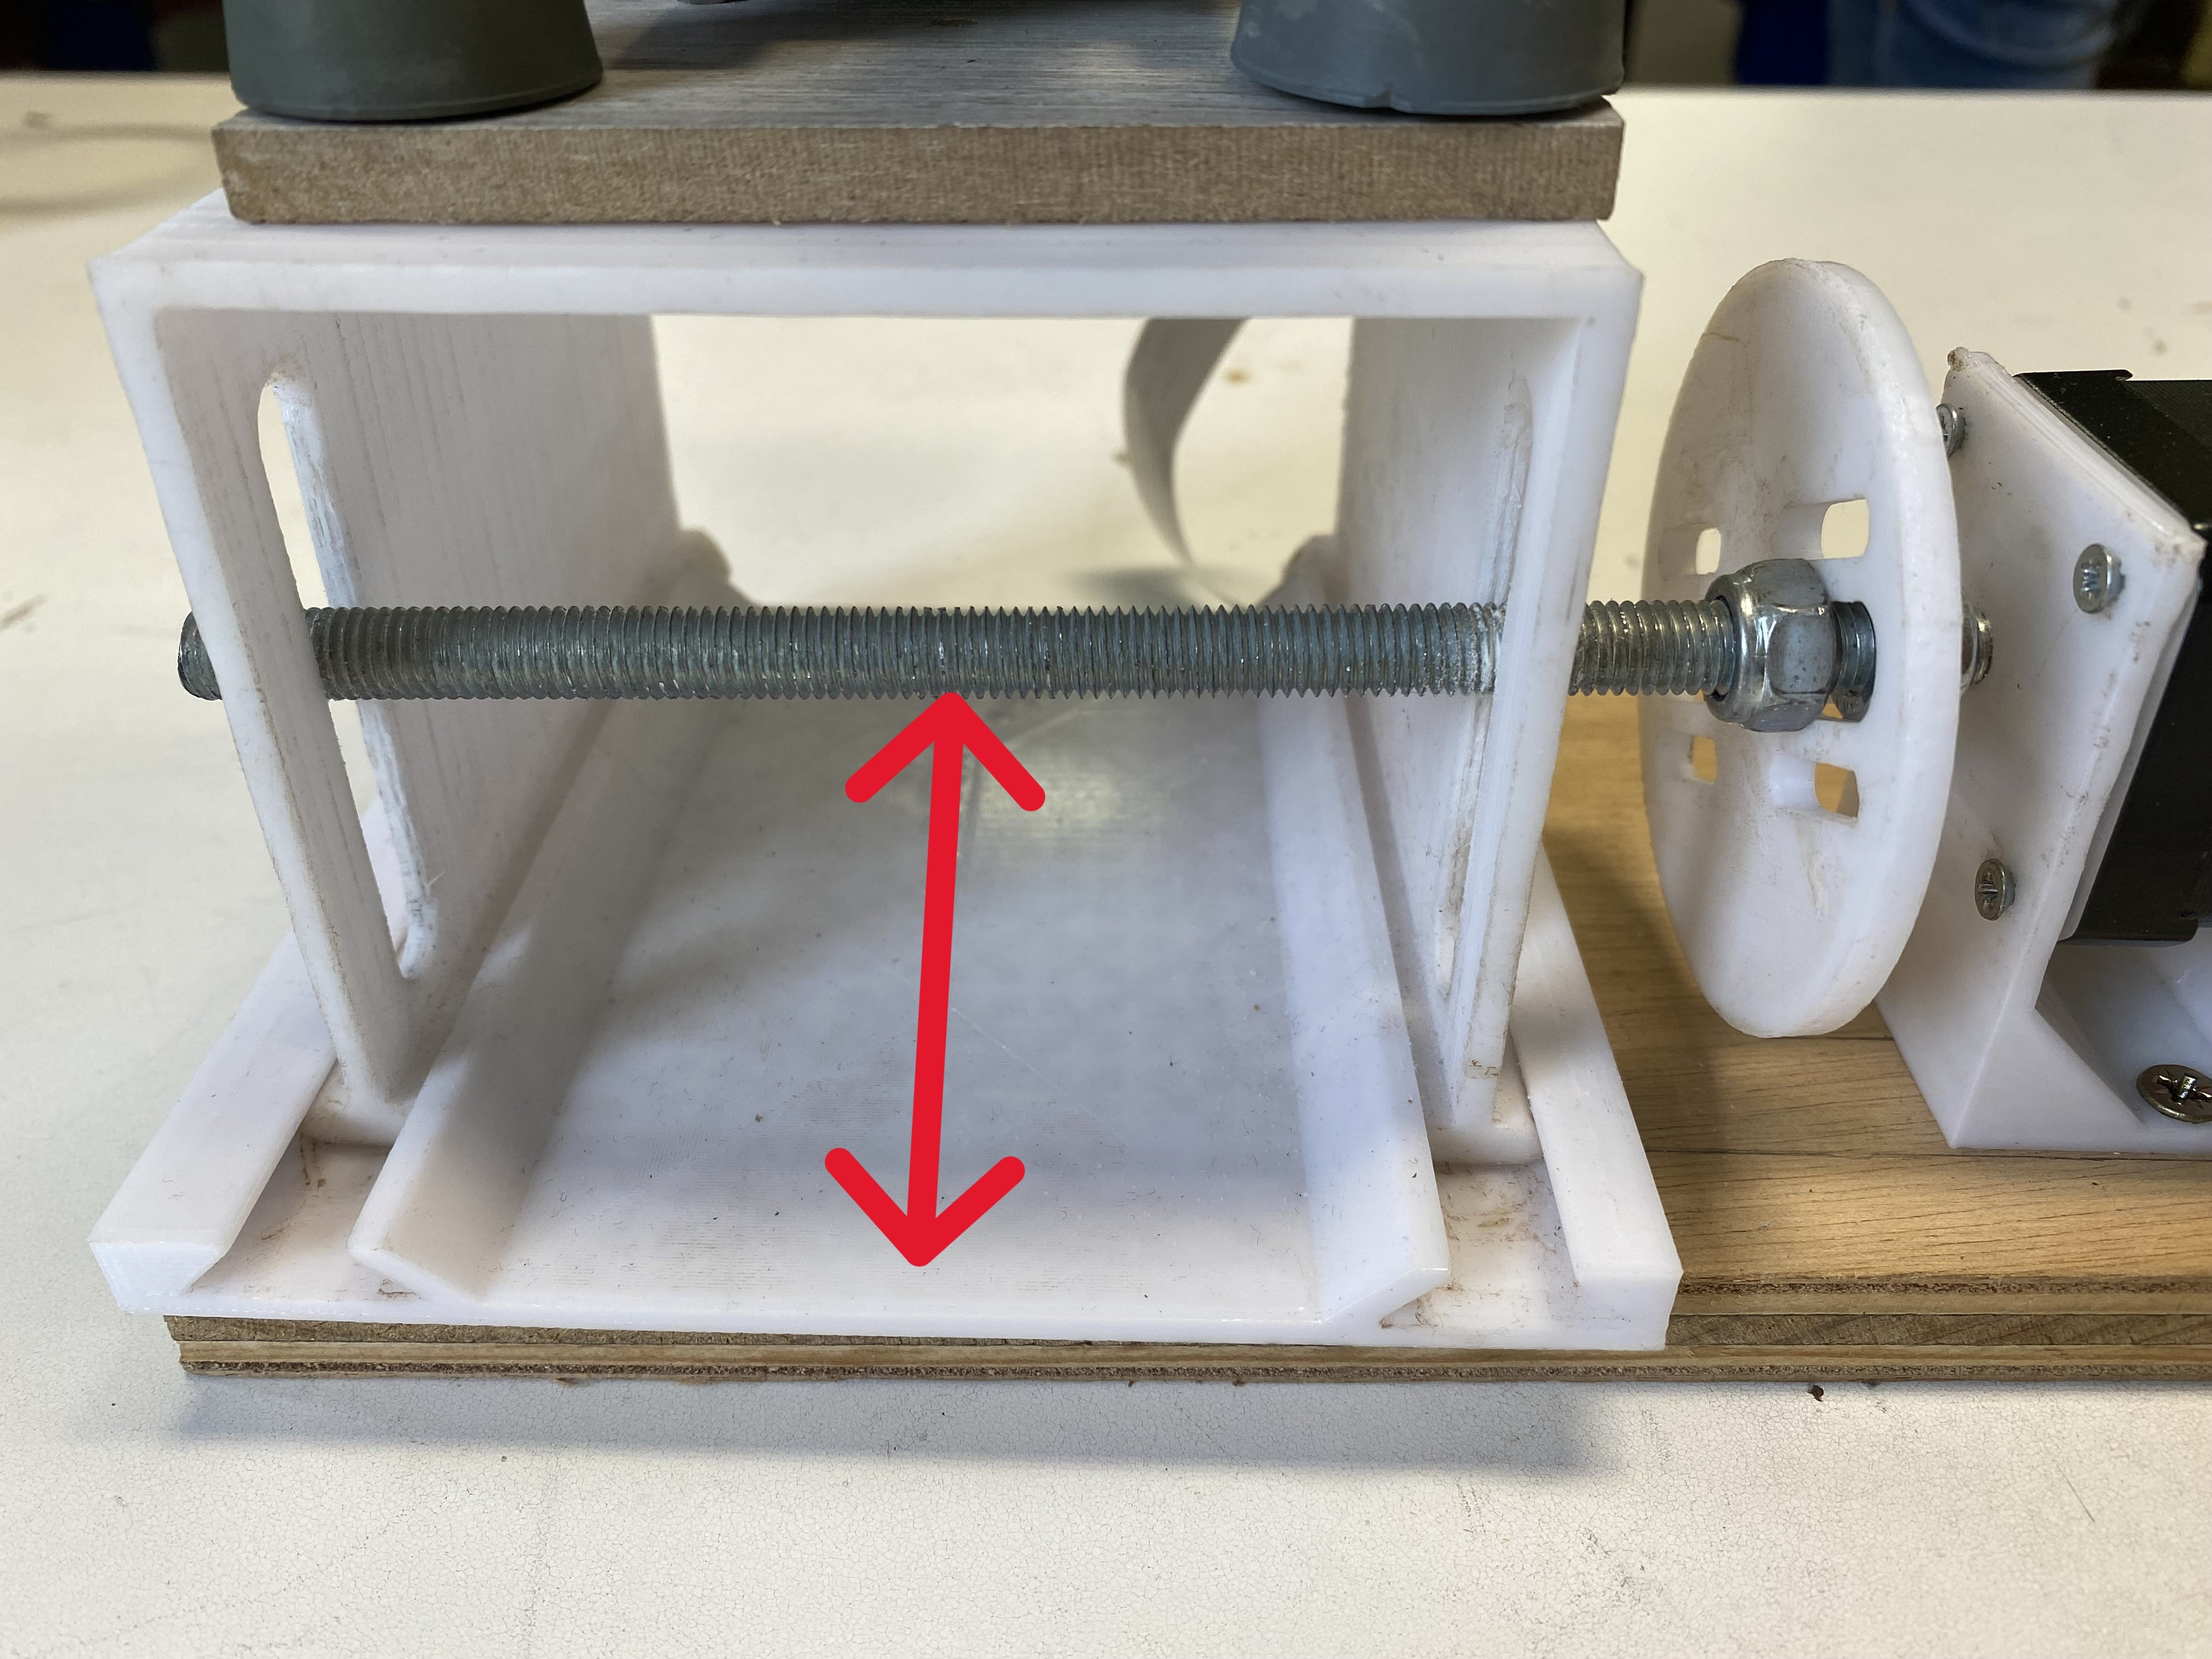
\includegraphics[width=\textwidth]{C:/Users/noebo/OneDrive/Documents/Prépa/TIPE TMD/Présentation/Photos comp/IMG_3367b-min.JPG}
					\caption{Mécanisme}
				\end{figure}
			\end{column}
			\begin{column}{0.5\textwidth}
				Avantages:
				\begin{itemize}
					\item\ Facilité pour fixer la structure
					\item Fréquence réglable \\
					\item Amplitude réglable 
				\end{itemize}
				\vspace{12pt}
				Inconvénients:
				
				\begin{itemize}
					\item Hystérésis
				\end{itemize}
			\end{column}
		\end{columns}
	Ajout du schéma cinématique du système
	\end{frame}
	
	
	
	\section{Mise en vibration de la maquette}
	
	\begin{frame}{Mise en vibration de la maquette}
		
		%schéma de la maquette avec des 2 accéléromètres
		\frametitle{Capteurs}
		\begin{columns}
			\begin{column}{0.25\textwidth}
				\begin{figure}
					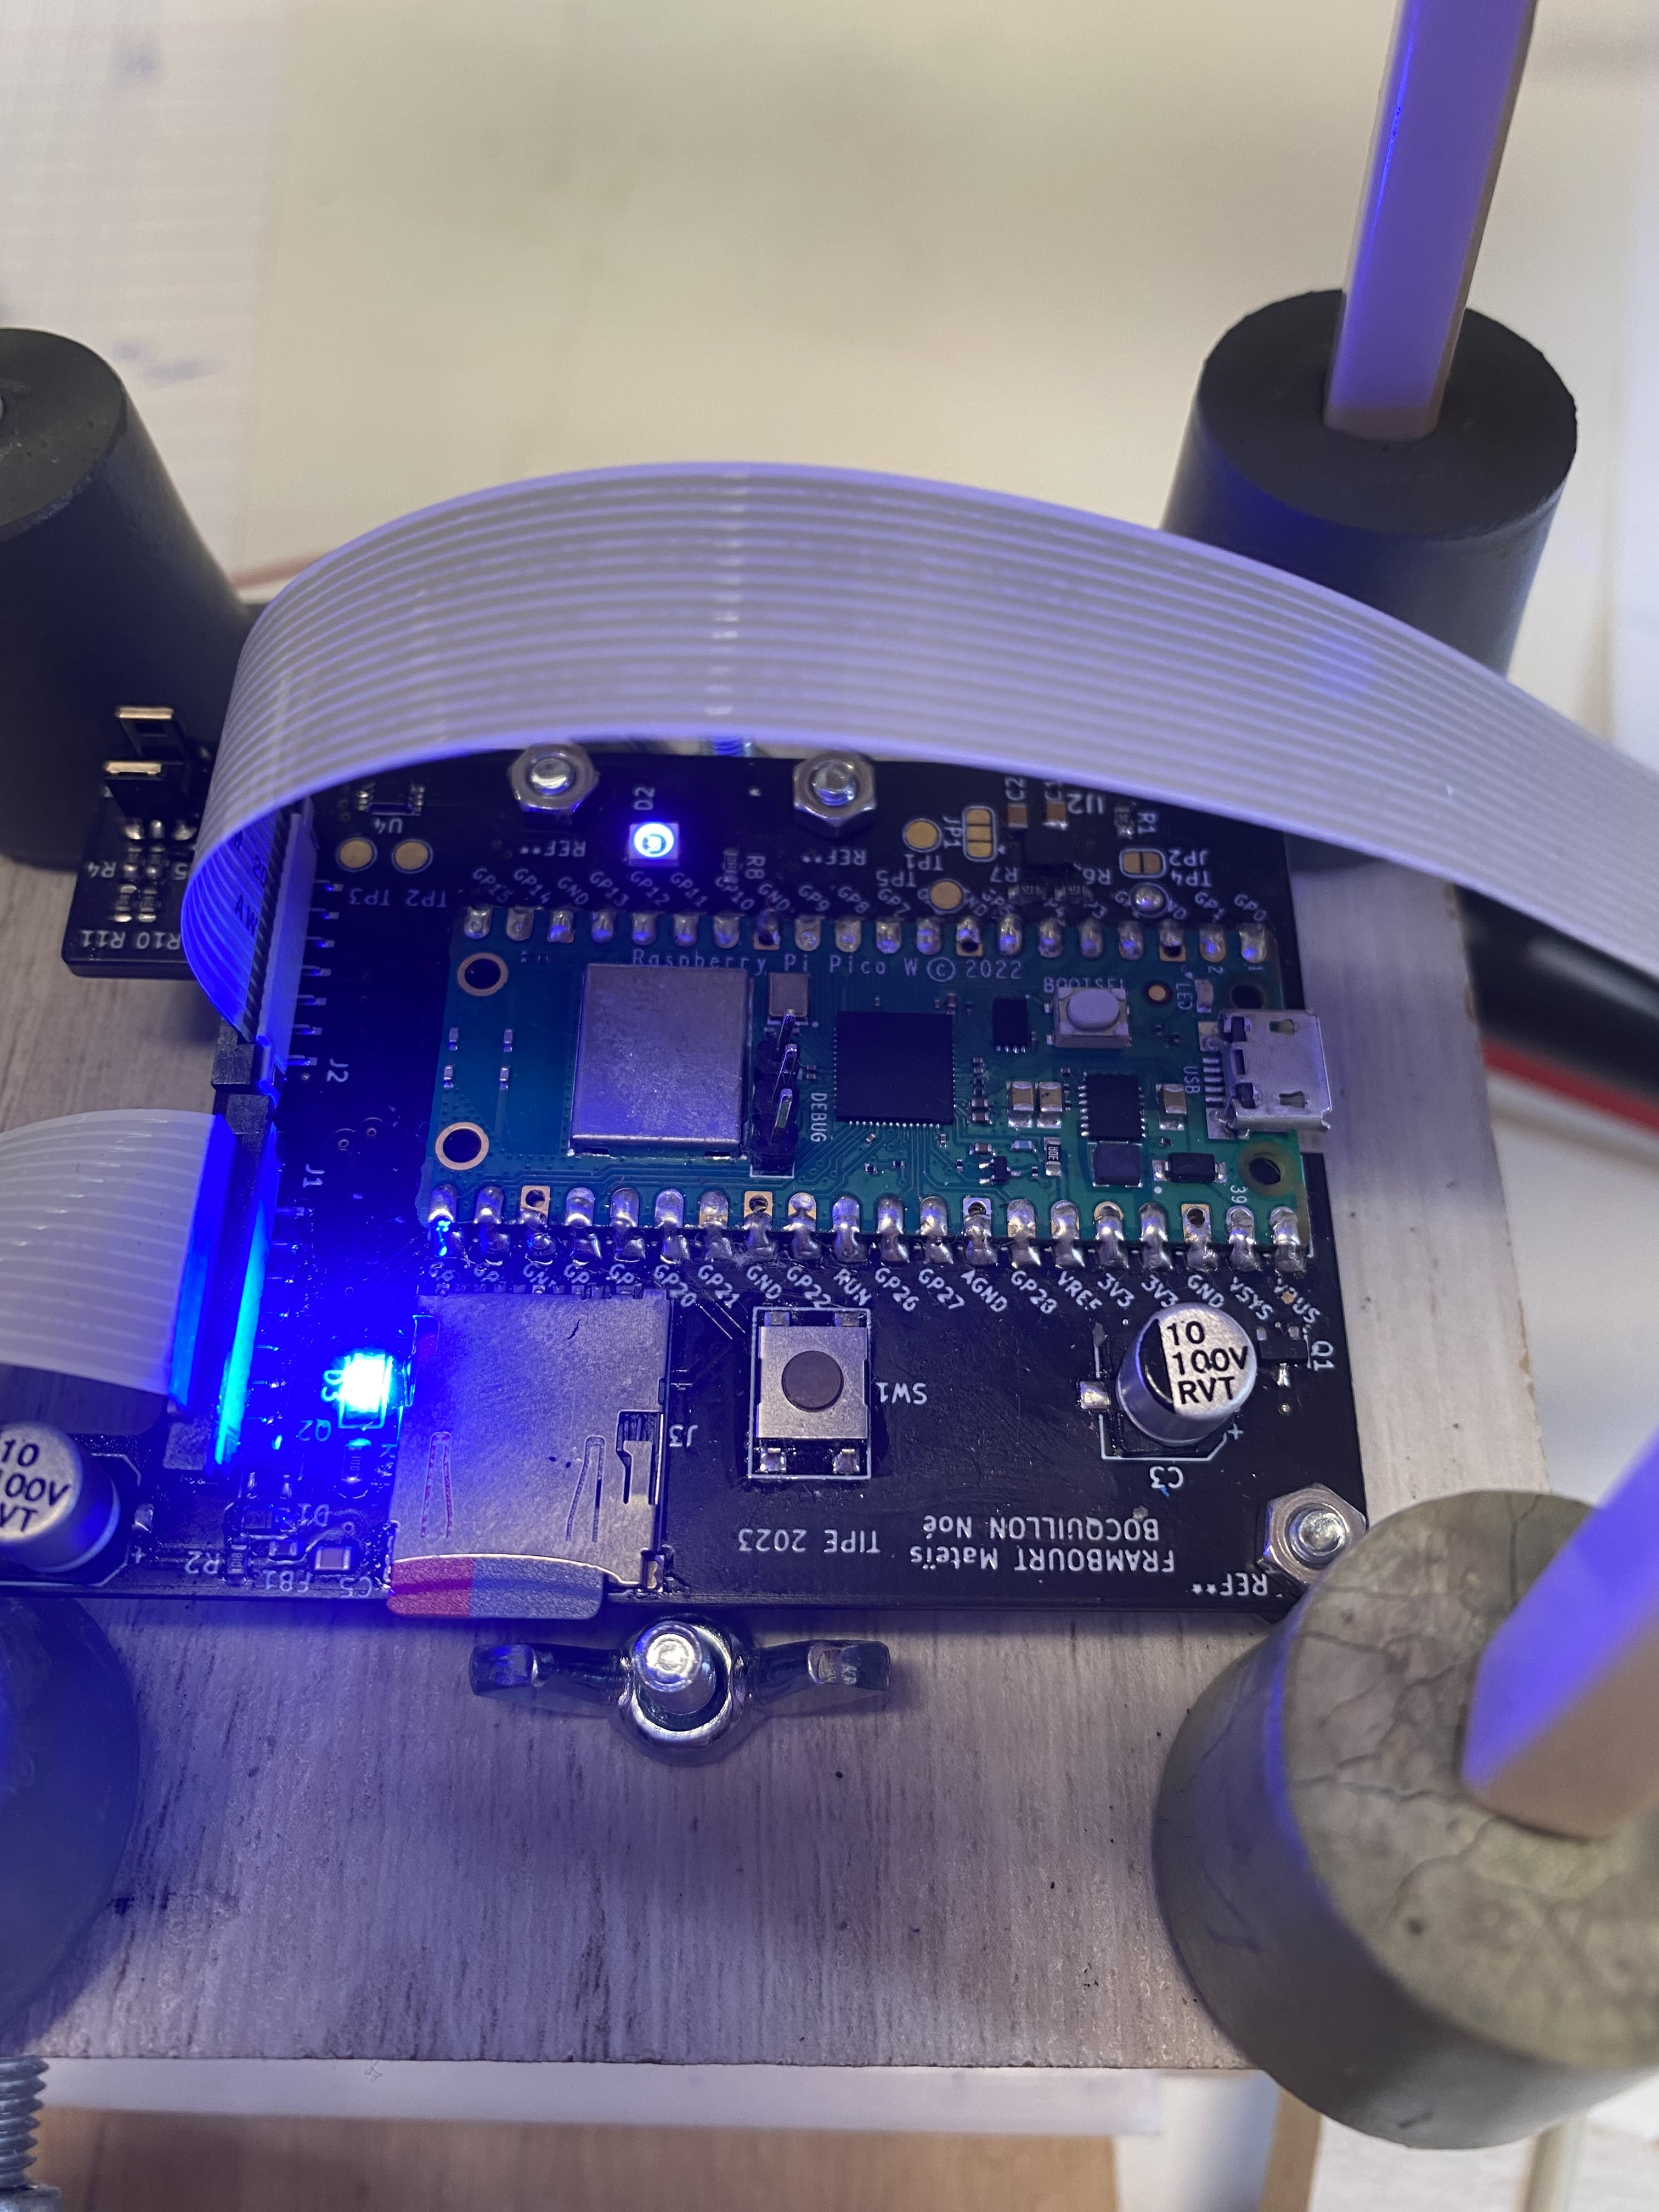
\includegraphics[width=\textwidth]{C:/Users/noebo/OneDrive/Documents/Prépa/TIPE TMD/Présentation/Photos comp/IMG_3378-min.JPG}
					\caption{Accéléromètre sur le socle}
				\end{figure}
			\end{column}
			\begin{column}{0.5\textwidth}
				\begin{figure}
					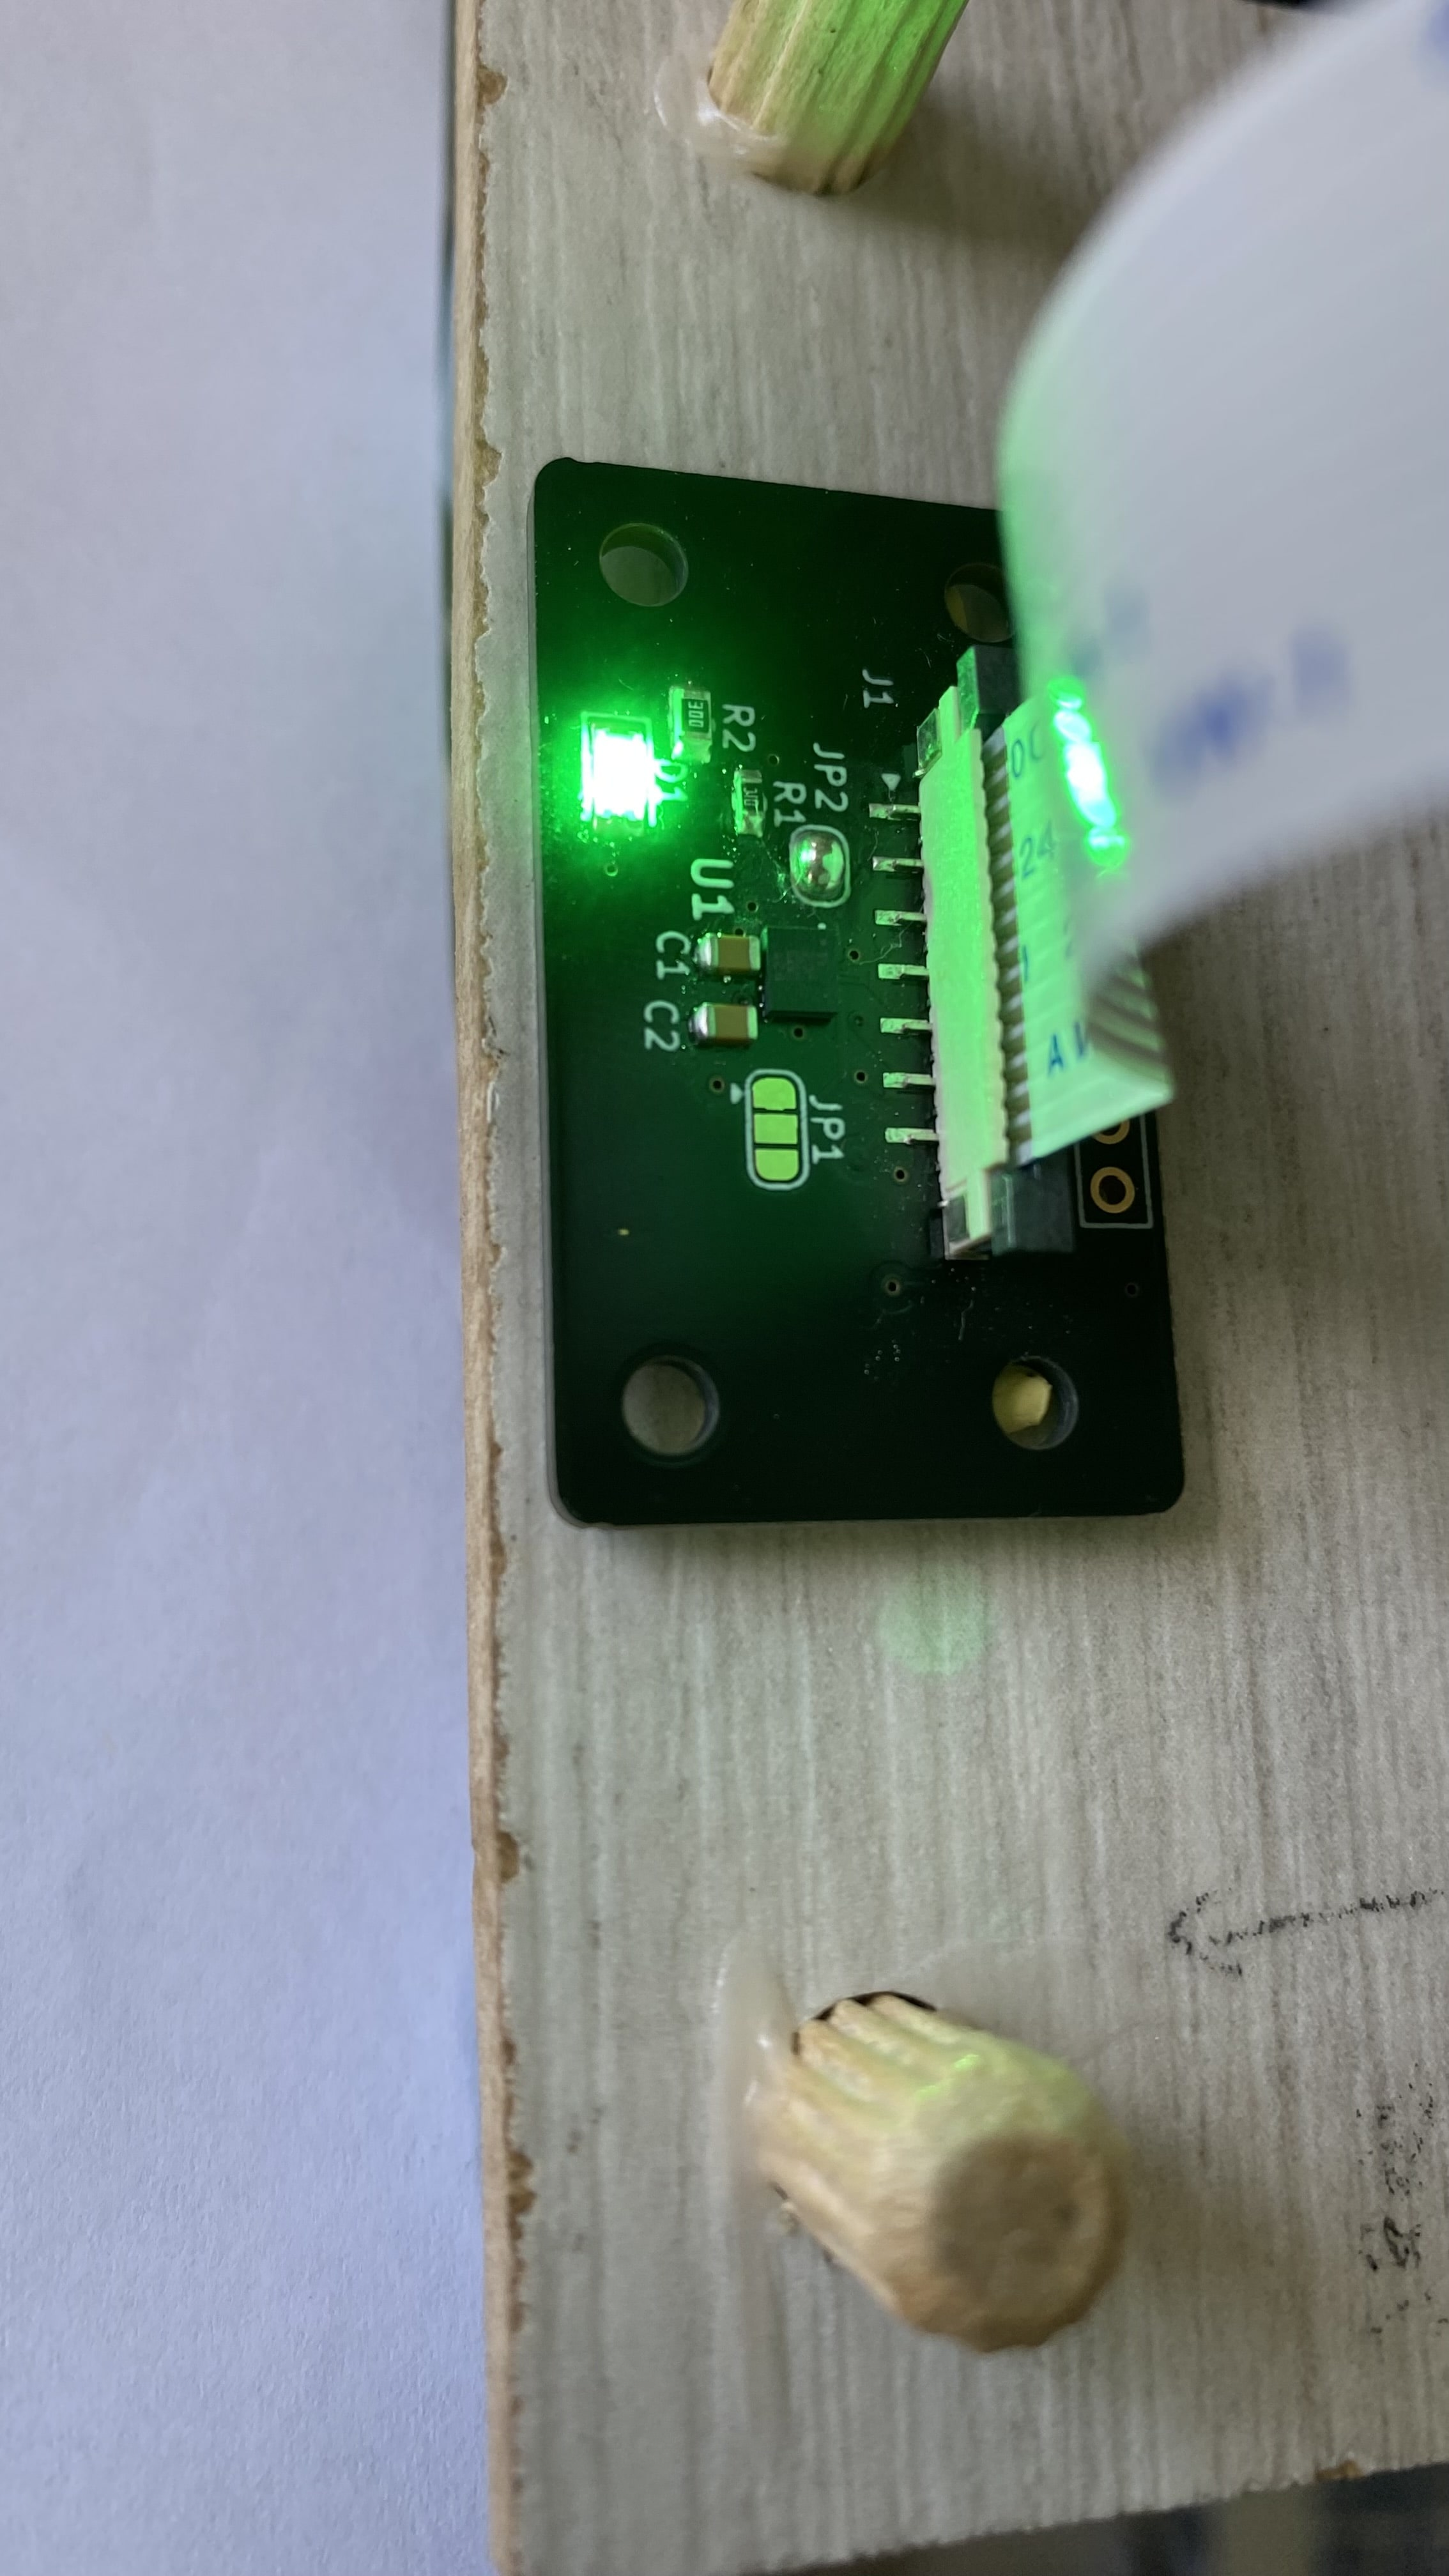
\includegraphics[width=0.5\textwidth]{C:/Users/noebo/OneDrive/Documents/Prépa/TIPE TMD/Présentation/Photos comp/IMG_E3393-min.JPG}
					\caption{Accéléromètre du haut}
				\end{figure}
			\end{column}
		\end{columns}
	Permet de tracer des diagrammes de Bode 
	\end{frame}
	
	\begin{frame}{Mise en vibration de la maquette}
		\frametitle{Première expérience:Réponse à une excitation sinusoïdale}
		\begin{columns}
			\begin{column}{0.35\textwidth}
				\alert{Simulation d'un séisme}
			\end{column}
			\begin{column}{0.5\textwidth}
				Conditions de l'expérience :
				\begin{itemize}
					\item Excentration la plus faible 
					\item Oscillations dans un seul plan
					\item Plage de fréquences :[0.5 hz;3.5 hz]
				\end{itemize}	
			\end{column}
		\end{columns}
		
		
		\begin{figure}
			Résultats:
			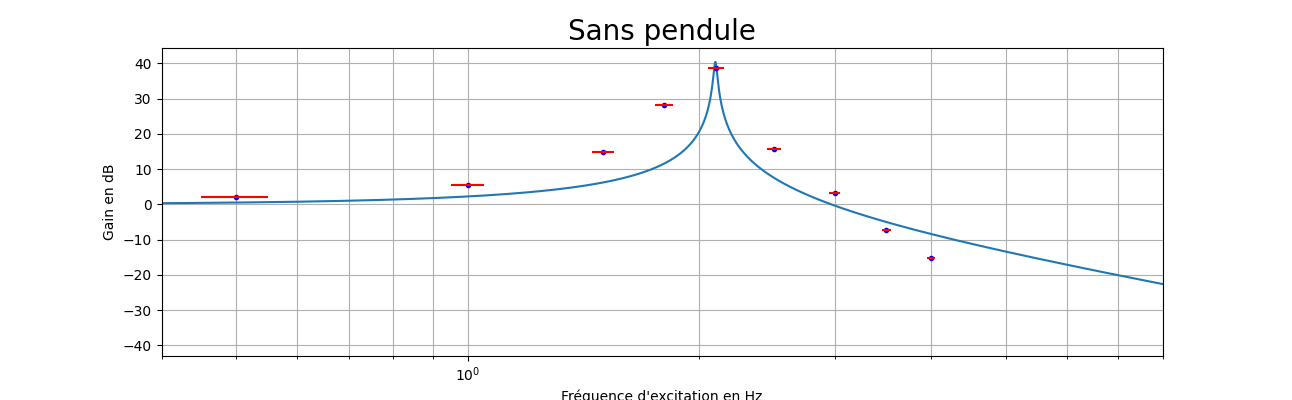
\includegraphics[scale=0.36]{C:/Users/noebo/OneDrive/Documents/Prépa/TIPE TMD/Présentation/Données pi/Sans pendule.png}
			
		\end{figure}
	\end{frame}
	
	
	
	\begin{frame}{Mise en vibration de la maquette}

		
		\begin{figure}
		\centering
		\includegraphics[scale=0.1]{C:/Users/noebo/OneDrive/Documents/Prépa/TIPE TMD/Présentation/Données pi/Masse de 100g à 3cm.png}
		
		
		\centering
		\includegraphics[scale=0.1]{C:/Users/noebo/OneDrive/Documents/Prépa/TIPE TMD/Présentation/Données pi/Masse de 100g à 5cm.png}
		\end{figure}
	\end{frame}
	
	\begin{frame}{Mise en vibration de la maquette}
		\frametitle{Première expérience:Réponse à une excitation sinusoïdale}
		\centering
		\includegraphics[scale=0.34]{C:/Users/noebo/OneDrive/Documents/Prépa/TIPE TMD/Présentation/Données pi/Masse de 100g à 9.4 cm.png}
		\\
		\vspace{12pt}
		Observations:
		\begin{itemize}
			\item Réduction de l'amplitude des oscillations
			\item Influence du centre de gravité du pendule
			\item Décalage de la fréquence de résonance  
		\end{itemize}
		
	\end{frame}
	
	\begin{frame}{}
		grpahiques: comparaison avec un modèle théorique pour valider ou refuter 
		revoir la forme des graphiques 
		mettre la phase
	\end{frame}
	\begin{frame}{}
		intro : plus scientifique, dissipation d'energie , antirésonnace, iterpeler avec les éléments des images,
	\end{frame}
	
	\begin{frame}{Mise en vibration de la maquette}
		\frametitle{Première expérience:Réponse à une excitation sinusoïdale}
		Variation de la masse du pendule:
		\begin{figure}
			\includegraphics[width=0.26\textwidth]{C:/Users/noebo/OneDrive/Documents/Prépa/TIPE TMD/Présentation/Photos/IMG_E3392.JPG}
			\caption{Pendule avec une masse de 73.2g}
		\end{figure}
	\end{frame}
	
	\begin{frame}{Mise en vibration de la maquette}
		\frametitle{Première expérience:Réponse à une excitation sinusoïdale}	
		\centering
		\includegraphics[scale=0.32]{C:/Users/noebo/OneDrive/Documents/Prépa/TIPE TMD/Présentation/Données pi/Masse de 100g à 5cm.png}
		
		
		\centering
		\includegraphics[scale=0.32]{C:/Users/noebo/OneDrive/Documents/Prépa/TIPE TMD/Présentation/Données pi/Masse de 73.2g à 5.5cm.png}
		
		
	\end{frame}
	
	
	
	
	\begin{frame}{Mise en vibration de la maquette}
		\frametitle{Deuxième expérience:Réponse à une excitation brève}
		\subtitle{bjr}
		\begin{columns}
			\begin{column}{0.5\textwidth}
				\alert{Simulation d'une rafale de vent}
				\begin{figure}
					\includegraphics[width=\textwidth]{C:/Users/noebo/OneDrive/Documents/Prépa/TIPE TMD/Présentation/Photos/IMG_E3390.JPG}
					\caption{Excitation brève}
				\end{figure}
			\end{column}
			\begin{column}{0.5\textwidth}
				Conditions de l'expérience :
				\begin{itemize}
					\item Dirac avec un ressort 
					\item Oscillations dans un seul plan
				\end{itemize}	
			\end{column}
		\end{columns}
	\end{frame}
	
	
	
	
	\begin{frame}{Mise en vibration de la maquette}
		\frametitle{Deuxième expérience:Réponse à une excitation brève}
		\centering Résultats
		\vspace{12pt}
		\begin{columns}[onlytextwidth]
			\begin{column}{0.33\textwidth}
				\centering
				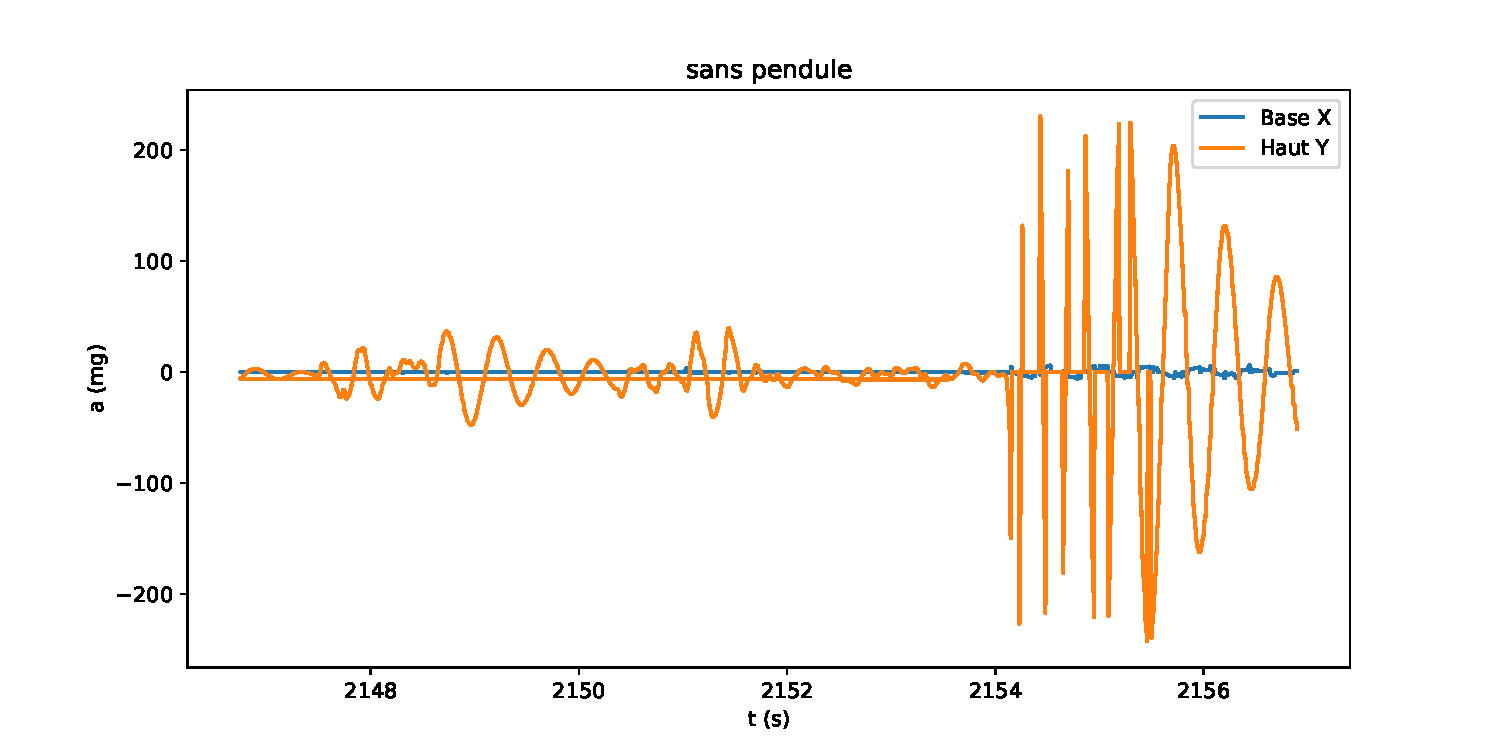
\includegraphics[width=1\textwidth]{C:/Users/noebo/OneDrive/Documents/Prépa/TIPE TMD/Présentation/Données pi/Coup de vent/sans pendule.pdf}
			\end{column}
			\begin{column}{0.33\textwidth}
				\centering
				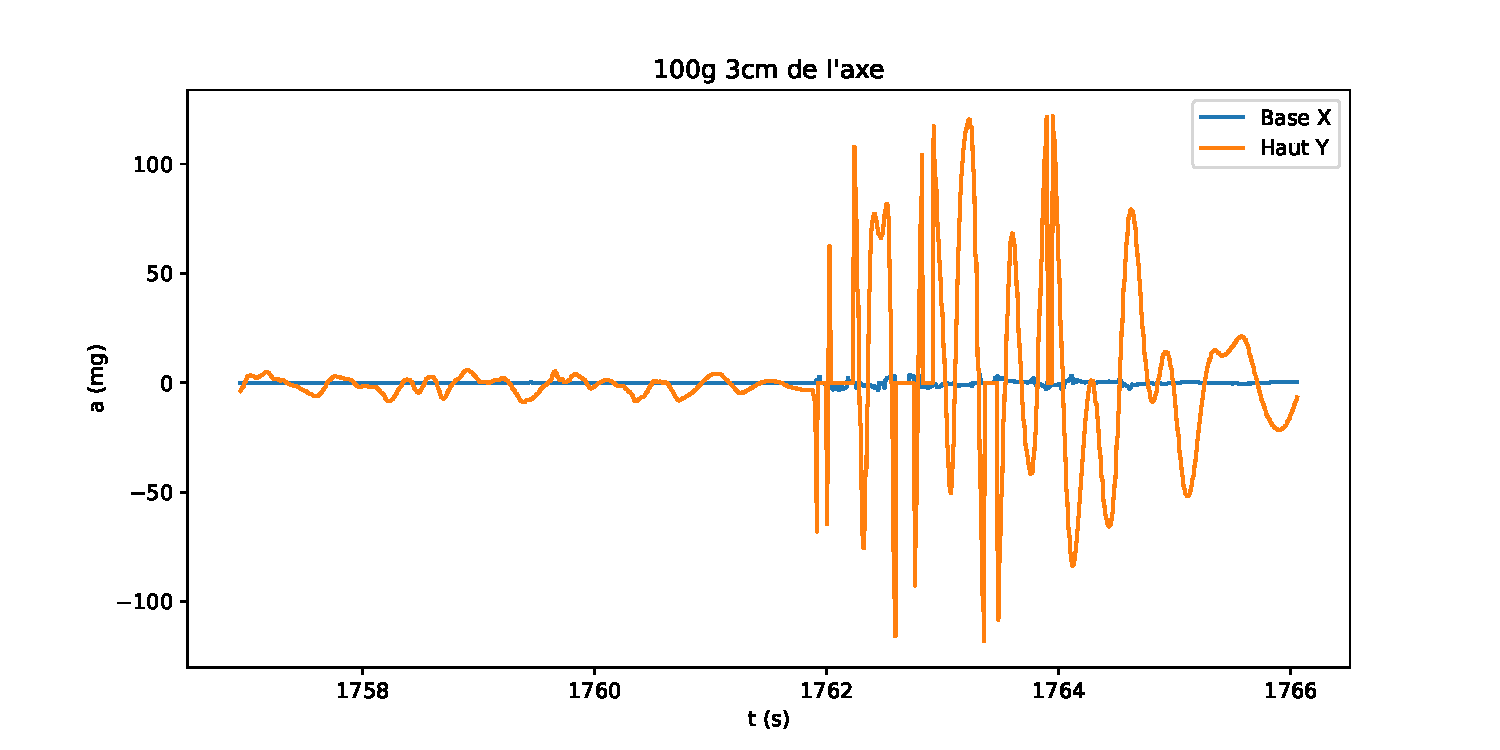
\includegraphics[width=1\textwidth]{C:/Users/noebo/OneDrive/Documents/Prépa/TIPE TMD/Présentation/Données pi/Coup de vent/100g 3cm de l'axe.pdf}
			\end{column}
			\begin{column}{0.33\textwidth}
				\centering
				\includegraphics[width=1\textwidth]{C:/Users/noebo/OneDrive/Documents/Prépa/TIPE TMD/Présentation/Données pi/Coup de vent/100g à 9.4 de l'axe.pdf}
			\end{column}
		\end{columns}
		\footnote{A modifier}
	\end{frame}
	
	
	
	
	
	\section{Élaboration d'un modèle théorique}
	\begin{frame}{Élaboration d'un modèle théorique}
		\frametitle{Modélisation du système}
		
		\begin{columns}
			\begin{column}{0.5\textwidth}
				\begin{figure}
					\centering
					\includegraphics[width=0.6\textwidth]{"C:/Users/noebo/OneDrive/Documents/Prépa/TIPE TMD/Présentation/Modélisation.png"}
					\caption{Modélisation du système}
				\end{figure}
			\end{column}
			\begin{column}{0.5\textwidth}
				\begin{itemize}
					\item $M_{2}$=Masse du pendule
					\item $M_{1}$=Masse de la tour
					\item K=Coefficient de raideur élastique (Baguettes + bouchons dans notre modèle)
					\item $C_{2}$= coefficient de frottement du pendule 
					\item $C_{1}$= coefficient de frottement de la tour
				\end{itemize}	
			\end{column}
		\end{columns}
		
	\end{frame}
	
	\begin{frame}{Élaboration d'un modèle théorique}
		\frametitle{Équations du système}	
		En appliquant le PFD à la tour sans pendule ni excitation\\ extérieure (correspond au dirac):
		\begin{equation}\label{key}
			\ddot{x} + \frac{C_{1}}{M_{1}}\dot{x}   +  \frac{k}{M_{1}} = 0
		\end{equation}\\
	\vspace{12pt}\\
		Période naturelle de la tour:\vspace{12pt} \\
		\begin{columns}
		\begin{column}{0.5\textwidth}
				$ T = 2\pi\frac{1}{\sqrt{\frac{K}{M_{1}}-\frac{C_{1}^2}{4M_{1}^2}}}$
		\end{column}
		\begin{column}{0.5\textwidth}
		 Expérimentalement $T= 0,5 s$
		\end{column}
	\end{columns}
	

		
	\end{frame}
%	\begin{frame}
	%	contenu...
	
%	$	Mesure de T et de C_{1} expérimentalement :\\ Obtention de la valeur de K$
%	\end{frame}
			
	
	\section{Conclusion}
	
	\begin{frame}{Limites du modèle}
		\begin{itemize}
			\item Dimensions peu assimilables au réel
			\item Élasticité trop importante 
		\end{itemize}	
		\vspace{12pt}
		
	\end{frame}
	
	%\begin{frame}{explications}
	%dissipation d'énergie dans le pendule , opposition de phases , rapport des pulsations naturelles
	%\end{frame}
	
	%\begin{frame}{limites}
	%	dimension peu adaptées (rapport de la taille et de la masse du pendule par rapport à la structure\\structure trop élastique qui entraine parfois des non linéarité à la fréquence de résonance )
	%\end{frame}
	
	%\begin{frame}{ce qu'on aurait aimé faire}
	%comparaison avec un modèle informatique\\
	%	plus de variations de paramètres\\
	%	mettre le pendule dans un fluide pour plus de viscosité
	%\end{frame}
	
	
	
	
	
	
	%\begin{frame}
	%	\frametitle{Annexe}
	%	Graphique et explication des mesures des coefficients de raideur
	%\end{frame}
\end{document}